\documentclass[11pt]{article}
\usepackage[a4paper, total={6.8in, 9.25in}]{geometry}
\usepackage{graphicx}
\graphicspath{ {./assets/images/output/} }
\usepackage{caption}
\usepackage[english]{babel}
\usepackage{float}
\usepackage{amsmath}
\usepackage{amssymb}
\usepackage{minted}
\usepackage{multicol}
\usepackage{array}
\usepackage{setspace}
\usepackage{placeins}
\usepackage{tcolorbox}
\usepackage{subcaption}

\definecolor{verbgray}{gray}{.95}
\setminted{
    bgcolor=verbgray,
    baselinestretch=1,
    fontsize=\footnotesize,
    linenos,
    breaklines=true,
    breakanywhere=true,
    xleftmargin=\parindent
}

\pagenumbering{gobble}
\begin{document}
\captionsetup{justification=centering}

% Custom cover page handles the title block
\input{dip_cover.tex}
\pagebreak

\tableofcontents
\pagebreak
\pagenumbering{arabic}

% EXPERIMENT 10
\begin{center}
    \section{Experiment 10: Boundary Extraction}
\end{center}

\subsection{Theory and Introduction}
Boundary extraction is a fundamental morphological operation used to identify the perimeter or outline of a binary object. The boundary of a set $A$, denoted as $\beta(A)$, can be obtained by first eroding $A$ with a suitable structuring element $B$, and then performing a set difference between the original set $A$ and its erosion \cite{gonzalez2018}.
$$
    \beta(A) = A - (A \ominus B)
$$
Where $\ominus$ denotes morphological erosion. By eroding the image with a $3 \times 3$ structuring element of 1s, the outermost layer of pixels of the object is stripped away. Subtracting this shrunken object from the original leaves only that outermost layer.

\subsection{Methodology}
A binary image containing a solid square shape was defined, and the boundary was extracted using morphological erosion and matrix subtraction.

\subsubsection{Matrix Definition}
A $6 \times 6$ binary image matrix $A$ was created containing a $4 \times 4$ solid block of 1s. A $3 \times 3$ Structuring Element (SE) $B$ consisting entirely of 1s was utilized to ensure a uniform 1-pixel thick boundary extraction.

\subsubsection{Python Implementation}
The SciPy $binary_erosion$ function was utilized to compute $A \ominus B$. The resulting eroded matrix was then subtracted from the original matrix $A$. The matrices were cast to integer types to perform the arithmetic subtraction $A - C$.

\begin{multicols}{2}
    \inputminted{python3}{./assets/lab10.py}
\end{multicols}

\subsection{Results}
The code successfully isolated the perimeter of the binary object.

\begin{figure}[H]
    \centering
    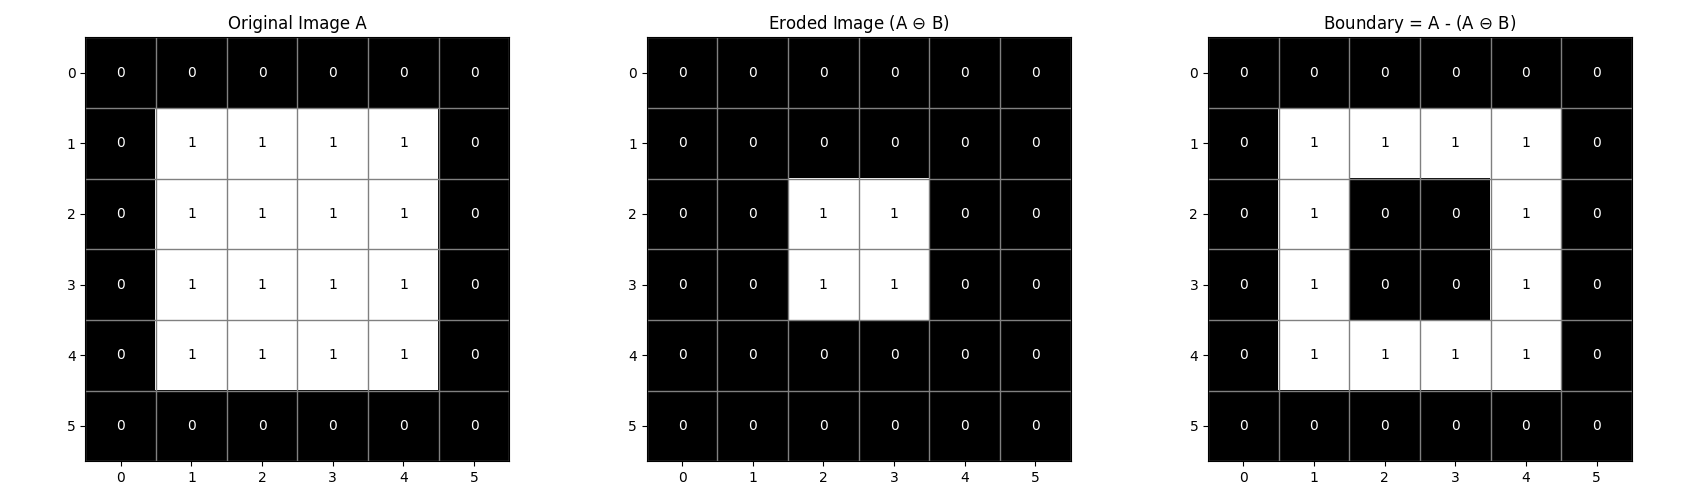
\includegraphics[width=\linewidth]{lab10_boundary.png}
    \caption{Boundary Extraction Process. Left: Original $4 \times 4$ object. Center: The object after erosion, reduced to a $2 \times 2$ core. Right: The extracted boundary, representing the difference between the first two matrices.}
    \label{fig:boundary}
\end{figure}

\subsection{Discussion}
The mathematical set difference proved effective for outline generation. The original object extended from index (1,1) to (4,4). After erosion with the $3 \times 3$ structuring element, only the inner core from index (2,2) to (3,3) survived, as these were the only pixels where the structuring element fit completely inside the object. Subtracting this $2 \times 2$ core from the original $4 \times 4$ object perfectly isolated the 1-pixel thick outer ring.

\subsection{Conclusion}
The mechanism of morphological boundary extraction was successfully validated. It was demonstrated that combining non-linear erosion with simple arithmetic subtraction is a robust method for isolating the perimeters of solid binary shapes.

\pagebreak
% EXPERIMENT 11
\begin{center}
    \section{Experiment 11: Region Filling}
\end{center}

\subsection{Theory and Introduction}
Region filling is a morphological algorithm used to fill holes in binary images. Given an image $A$ containing boundaries, and a point $p$ inside a boundary, the goal is to fill the entire enclosed region with 1s. This is achieved iteratively by dilating a seed point and constraining its growth so it does not spill past the boundary. The recursive equation is \cite{gonzalez2018}:
$$
    X_k = (X_{k-1} \oplus B) \cap A^c
$$
Where $X_0$ is the initial seed point, $B$ is a cross-shaped structuring element, and $A^c$ is the complement of the boundary image. The iteration terminates when $X_k = X_{k-1}$. The final filled image is the union of the original boundary and the filled region ($A \cup X_k$).

\subsection{Methodology}
A hollow square boundary was defined, an internal seed point was selected, and the iterative morphological filling algorithm was implemented.

\subsubsection{Matrix Definition}
A $7 \times 7$ binary image $A$ was defined containing a continuous 1-pixel thick boundary outline. A cross-shaped $3 \times 3$ Structuring Element $B$ was used to prevent diagonal spilling. An initial seed matrix $X_0$ was created with a single 1 at coordinate (3,3), strictly inside the boundary.

\subsubsection{Python Implementation}
A $while True$ loop was constructed to execute the recursive equation. In each iteration, the current region $X_{prev}$ was dilated using $binary_dilation$ and immediately intersected (logical AND) with $A^c$. The loop was broken when $np.array_equal$ confirmed the region had stopped growing.

\begin{multicols}{2}
    \inputminted{python3}{./assets/lab11.py}
\end{multicols}

\subsection{Results}
The iterative algorithm successfully flooded the internal region without breaching the boundary walls.

\begin{figure}[H]
    \centering
    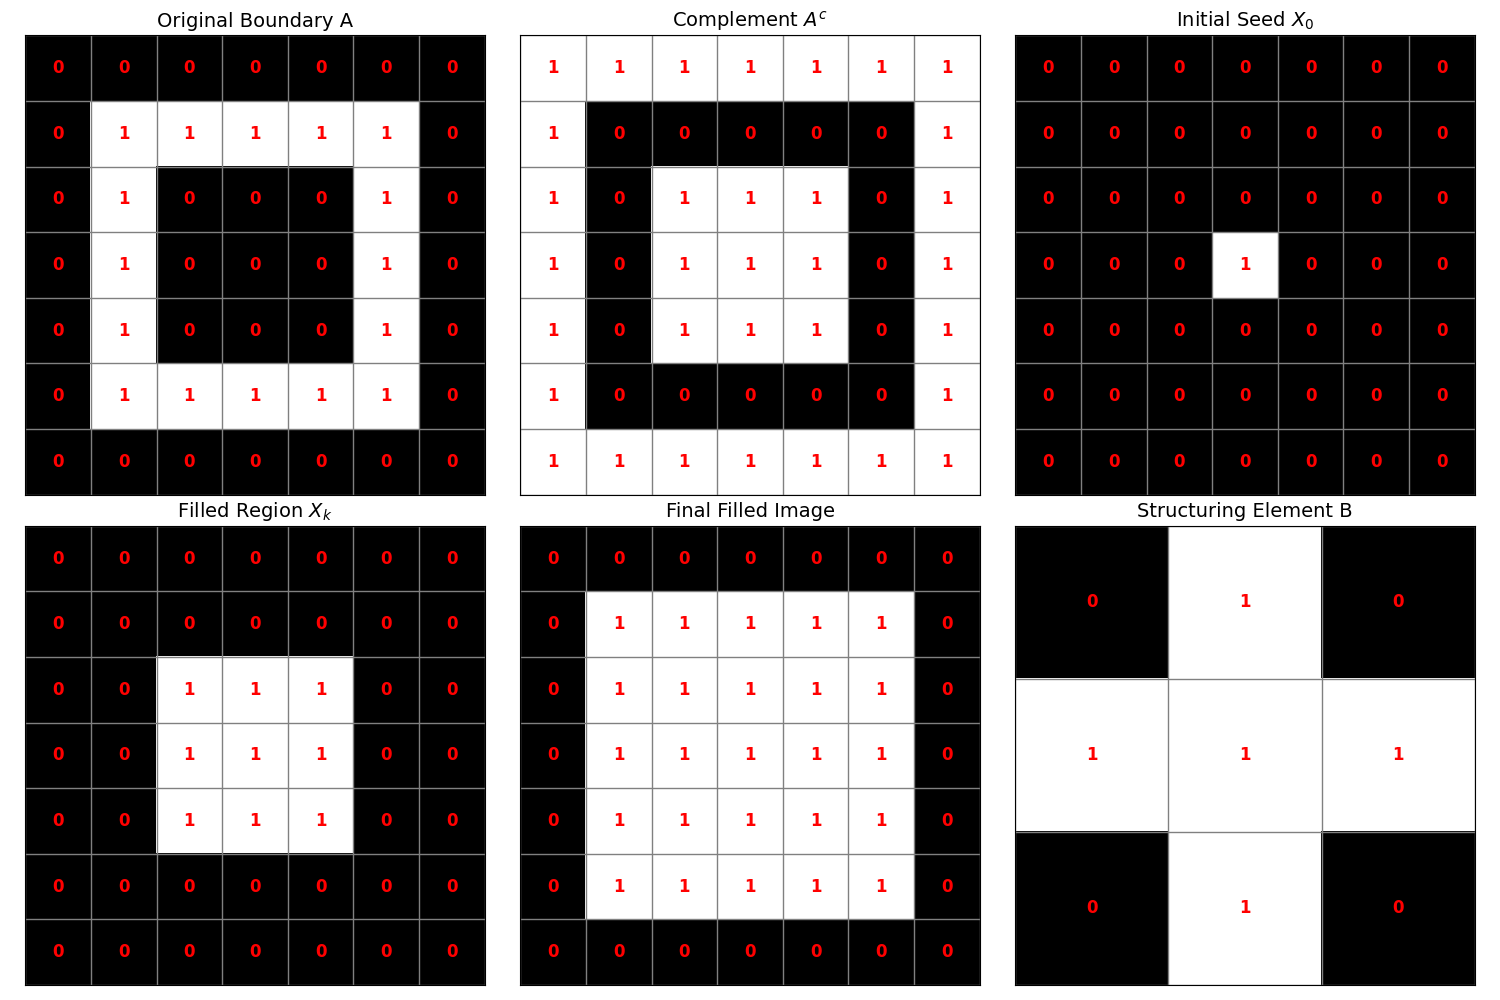
\includegraphics[width=\linewidth]{lab11_fill.png}
    \caption{Region Filling Process. The initial seed $X_0$ is iteratively dilated and constrained by $A^c$ until it fills the inner void. The final image is the union of $A$ and $X_k$.}
    \label{fig:fill}
\end{figure}

\subsection{Discussion}
The importance of the $A^c$ constraint was clearly demonstrated. The cross-shaped structuring element $B$ caused the seed point to grow horizontally and vertically. Without the intersection with $A^c$, the dilation would have eventually filled the entire $7 \times 7$ matrix. By continuously applying $A^c$, any dilated pixels that overlapped with the original boundary (where $A^c = 0$) were immediately erased, effectively using the boundary as an impassable wall. The process naturally converged when the entire hollow space was occupied.

\subsection{Conclusion}
The theoretical algorithm for morphological region filling was successfully implemented. It was verified that constrained iterative dilation from a known internal seed point is a reliable method for filling enclosed spaces within binary boundaries.

\pagebreak
% EXPERIMENT 12
\begin{center}
    \section{Experiment 12: Connected Components Extraction}
\end{center}

\subsection{Theory and Introduction}
Extracting connected components is essential for automated image analysis, object counting, and classification. The algorithm isolates a complete, contiguous object from a complex binary image given a single known point on that object. The recursive equation is mathematically similar to region filling \cite{gonzalez2018}:
$$
    X_k = (X_{k-1} \oplus B) \cap A
$$
Where $X_0$ contains the initial point, $B$ is the structuring element determining connectivity (4-connected or 8-connected), and $A$ is the original image. Unlike region filling which intersects with the complement, this algorithm intersects with the original image $A$ to constrain the growth strictly to existing foreground pixels. Iteration stops when $X_k = X_{k-1}$.

\subsection{Methodology}
A binary matrix with multiple separate objects was defined. A seed point was placed on one specific object, and the iterative extraction algorithm was applied.

\subsubsection{Matrix Definition}
A $7 \times 7$ binary image $A$ was defined containing an irregular L-shaped object and a separate, isolated point. An 8-connected Structuring Element $B$ (a $3 \times 3$ matrix of all 1s) was utilized. A seed point was placed at coordinate (2,3), which lies on the L-shaped object.

\subsubsection{Python Implementation}
The implementation mirrors the region-filling loop. The $binary_dilation$ function was applied to the seed matrix, and the result was intersected (logical AND) with the original image $A$. The loop terminated upon convergence.

\begin{multicols}{2}
    \inputminted{python3}{./assets/lab12.py}
\end{multicols}

\subsection{Results}
The algorithm successfully isolated the contiguous L-shaped object while ignoring the disconnected noise point.

\begin{figure}[H]
    \centering
    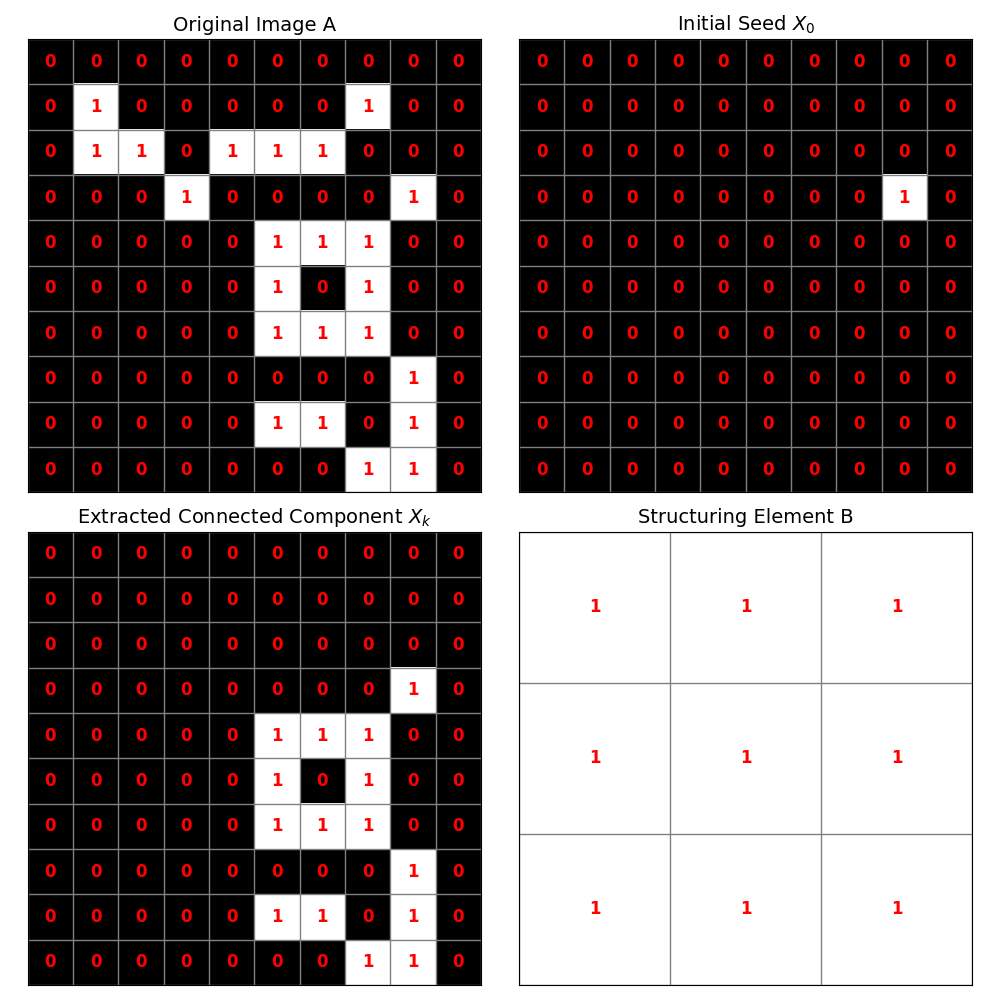
\includegraphics[width=0.8\linewidth]{lab12_connected.png}
    \caption{Connected Components Extraction. The seed $X_0$ iteratively grows along the foreground pixels of $A$. The isolated point at (1,5) in the original image is successfully ignored.}
    \label{fig:connected}
\end{figure}

\subsection{Discussion}
The distinction between the intersection constraints was highlighted. By applying the logical AND operation with the original image $A$, the dilated seed was only allowed to survive where foreground pixels already existed. Over successive iterations, the seed propagated through the entire L-shaped structure. Because the structuring element $B$ could not bridge the gap of zeros between the L-shape and the isolated point at (1,5), that point was never reached by the dilation process and was effectively filtered out of the final component $X_k$.

\subsection{Conclusion}
The morphological extraction of connected components was successfully validated. It was demonstrated that iterative dilation constrained by the original image bounds is an effective method for isolating specific contiguous objects from multi-object binary images.

% REFERENCES
\pagebreak
\bibliographystyle{IEEEtran}
\renewcommand{\bibname}{References}
\addcontentsline{toc}{section}{References}
\bibliography{ref}

\end{document}